In this section the \textbf{K}nowledge \textbf{D}iscovery \textbf{M}odel-\textbf{R}efactoring \textbf{E}nvironment (KDM-RE) is presented. In Figure~\ref{fig:process} we depict the overall process of our technique which was adapted based on the horseshoe modernization model. It is split into three parts, they are: (\textit{i}) Reverse Engineering, (\textit{ii}) Refactorings and (\textit{iii}) Forward Engineering. Furthermore, our process is divided into six levels. Firstly, the user starts the process in the \textbf{Level-0} by choosing an eclipse project which contains the source-code to realize the refactorings.  After that, into \textit{Level-1} it is need to transform the source-code into a Platform-Specific Model (PSM). This PSM is an instance of the source-code which represents all abstraction of the source-code, in Figure~\ref{fig:discovery_java_model} illustrates how to get the instance of this PSM having as input an eclipse project. This PSM represents an Abstract Syntax Tree (AST) that represents the syntactic struct of Java source code.

\begin{figure}[!ht]
\centering
  % Requires \usepackage{graphicx}
  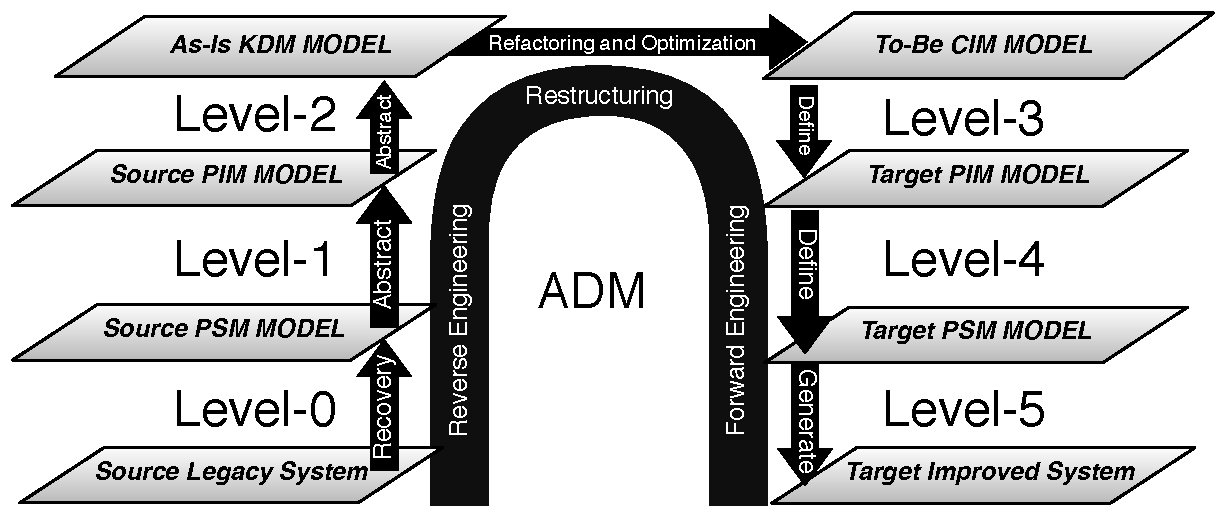
\includegraphics[width=11cm, height=3.8cm]{figure/processoDaFerramenta}
\caption{KDM-RE Process}
\label{fig:process}
\end{figure} 

As long as the user has triggered the earlier step, the next one is to transform the PSM to a Platform-Indented Model (PIM) based on the KDM. Therefore, in this step the tool performs a set of model-to-model to get an instance of the KDM which represents the systems ``AS-IS''. In Figure~\ref{fig:discovery_kdm_model} depicts how to get the instance of the KDM based on the earlier PSM.

\begin{figure}
\centering
\begin{minipage}{.5\textwidth}
  \centering
  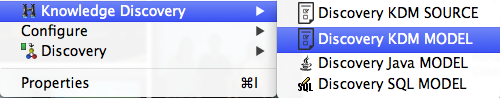
\includegraphics[width=6cm\linewidth]{figure/discovery_kdm_model}
  \captionof{figure}{Discovery Java Model}
  \label{fig:discovery_java_model}
\end{minipage}%
\begin{minipage}{.5\textwidth}
  \centering
  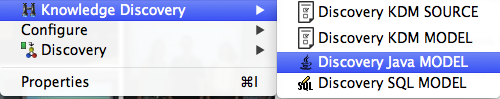
\includegraphics[width=6cm\linewidth]{figure/discovery_java_model}
  \captionof{figure}{Discovery Java Model}
  \label{fig:discovery_kdm_model}
\end{minipage}
\end{figure}